\section{High Energy Astrophysics}

\begin{sectionauthor}
    Yasmeen Asali (Yale University) \\
    Michelle Gurevich (King's College London) \\
    Dr. Emily Lichko (The University of Chicago) \\
    Julie Malewicz (Georgia Institute of Technology) \\
    Samantha Pagan (Yale University) \\
    Emily Simon (The University of Chicago)
\end{sectionauthor}
\vspace{20pt}


\subsection{Astrophysical Plasmas}

While we are mainly familiar with three states of matter in our daily lives-- liquids, solids, and gasses-- there exists a fourth state of matter called a plasma. Plasmas are electrically charged gasses, meaning that the molecules of the gas have been pulled apart into positively and negatively charged components (for example: removing one negatively-charged electron from a hydrogen atom will leave behind a positively charged proton). Even though most gasses we encounter on Earth are neutral, in outer space where things are very hot and energetic, most gasses are electrically charged and are therefore called plasmas. 

It's important to understand how plasmas work in order to study highly energetic astrophysical phenomena such as solar winds, supernovae, and the disks of superheated matter that are captured by black holes (accretion disks). The key concept is that plasmas are full of electrically charged particles which are susceptible to electricity and magnetism. In the presence of a strong electric or magnetic field, particles can get huge energy boosts, have their trajectories through space reoriented, or even collide with one another and form other particles. 

On Earth, we can create plasmas in the lab to study their behaviors, but it can be challenging or impossible to inject enough energy or to make large enough magnets to match the scales that we see in space. We can also study what happens when plasmas from space interact with the Earth's atmosphere. Periodically the sun will release large bursts of energized particles (called the solar wind) towards the Earth which are deflected by the Earth's magnetic field and funneled into the North and South poles. When these particles collide with atoms in the air like hydrogen, nitrogen, or carbon dioxide, they transfer their energy and cause the atmospheric molecules to fluoresce in bright colors. This is known as the aurora borealis in the Northern hemisphere and the aurora australis in the Southern hemisphere.

\subsection{Cosmic Rays} 

The most energetic particles in the universe are called ``cosmic rays''. While their name may make them sound like a wave, in reality they are made of ions and electrons, the positively and negatively charged particles that work together to make electricity run through our homes. Because they are so energetic, even a small number of cosmic rays, each of which is the size of an atom, roughly $10^{-10}$ m, can play a huge role in the evolution of astrophysical objects like galaxies that are roughly $10^{20}$ m. 

One of the biggest questions that we still don't understand about cosmic rays is how they get to be so fast. One of the most likely theories involves supernova remnants, the remains of stars that have exploded. The cosmic rays are ejected from the explosion, and then bounce back and forth over the boundary between the inside and the outside of the supernova remnant, picking up energy each time they bounce. one could imagine an air hockey puck, hit harder and harder each time it nears the other player, until it is hit so far it flies off the table. For the cosmic rays, eventually they are moving so fast that they can't be contained near the boundary of the supernova remnant, and they shoot out into the rest of the universe.

\subsection{Astroparticle Physics}

Astroparticle physics is a relatively new branch of study that began in the early 1900s with the discovery that at higher latitudes in Earth’s atmosphere, more particles exist that knock off electrons from other particles (called ionization). Scientists famously first observed this by measuring ionization at the top of the Eiffel Tower and later at higher altitudes in the atmosphere during air balloon flights. This discovery demonstrated that high-energy particles called cosmic rays travel to Earth from the cosmos. In astroparticle physics today, scientists study cosmologically created high-energy particles of many types (e.g. neutrinos, high-energy gamma rays, cosmic rays). Studying these particles enables discoveries about fundamental particles, cosmology, astronomy, and astrophysics–––making it a truly interdisciplinary area of study. 

In particle physics, The Standard Model, colloquially called the ``Theory of Everything,'' is an encompassing theory that impressively explains and predicts the interactions of many fundamental particles like electrons and quarks (these make up protons and neutrons). Based on the Standard Model, physicists have even predicted the existence of new particles like the Higgs Boson before it was discovered experimentally. Many particle physics experiments occur at particle colliders, like the Large Hadron Collider (LHC) at CERN in Geneva, Switzerland. Here, particles are accelerated to high energies and then smashed together. Rather than using colliders, astroparticle physicists study fundamental particles that travel to Earth from various sources in the cosmos. These particles can provide information about our universe as well as be used to study the properties of fundamental particles themselves. Some cosmological sources accelerate particles to far greater energies than is currently possible with human-made instruments. For example, the LHC's highest energy protons produced at CERN have 10$^{12}$ eV, while cosmic rays containing protons have 10$^{20}$ eV. (An eV is a unit of energy equal to moving one electron through a 1 Volt potential difference, which is about that of a AA battery.)


Some of the main unanswered questions in astroparticle physics are: What are dark energy and matter? Why is there more matter than antimatter in our universe? How did the universe evolve? What are the properties of fundamental particles like neutrinos? How are cosmic rays created?

Particles studied in the field include:
\begin{itemize}
    \item High-energy gamma rays: Gamma rays are the highest-energy form of light and, therefore also have the shortest wavelength. Astronomical objects like black holes, neutron stars, and supernovae create gamma rays. 
    \item Neutrinos: Neutrinos are extremely low-mass particles that rarely interact with other types of matter. They are often described as "ghost-like" particles and often pass through the Earth without interacting. Particle astrophysics experiments studying neutrinos emitted from the Sun were essential to the Nobel Prize-winning discovery that neutrinos strangely oscillate between flavors, a property of particles, which contradicted the Standard Model of particle physics.
    \item Cosmic rays: Energetic particles made of ions, electrons, protons, and gamma rays. 
    \item Dark matter candidates: What dark matter is (e.g., a particle, wave, black holes) is still unknown and undiscovered. However, multiple theories of what dark matter could be predict that dark matter particles could be created in the Sun and the universe or exist throughout our galaxy and commonly travel through Earth. 
\end{itemize}

The scientific instruments used in astroparticle physics are diverse and varying, too. The particle of interest determines the detectors and materials best suited for an experiment or observatory. Some astroparticle searches are built in underground laboratories like Xenon1T in Laboratori Nazionali del Gran Sasso (LNGS) in Italy. LNGS is located under a mountain and covered by 1,400 m of rock. The rock above underground laboratories shields experiments from some cosmological-originating particles like low-energy cosmic rays so scientists can more sensitively study particles like high-energy neutrinos and dark matter, which commonly pass through mountains. 

IceCube, the largest neutrino observatory in the world, is built inside the ice at the South Pole in Antarctica, at depths of almost 2,500 meters. Some of IceCubes' searches use the entire Earth as a shield for particles, so particles like high energy neutrinos (up to 10$^{21}$ eV in energy) that rarely interact with matter and commonly pass through the Earth can be carefully studied. In June 2023, IceCube released a first image of our galaxy, the Milky Way, from high-energy neutrinos\footnote{\href{https://icecube.wisc.edu/news/press-releases/2023/06/our-galaxy-seen-through-a-new-lens-neutrinos-detected-by-icecube/}{https://icecube.wisc.edu/news/press-releases/2023/06/our-galaxy-seen-through-a-new-lens-neutrinos-detected-by-icecube}}.

\begin{figure}[h!]
    \centering
    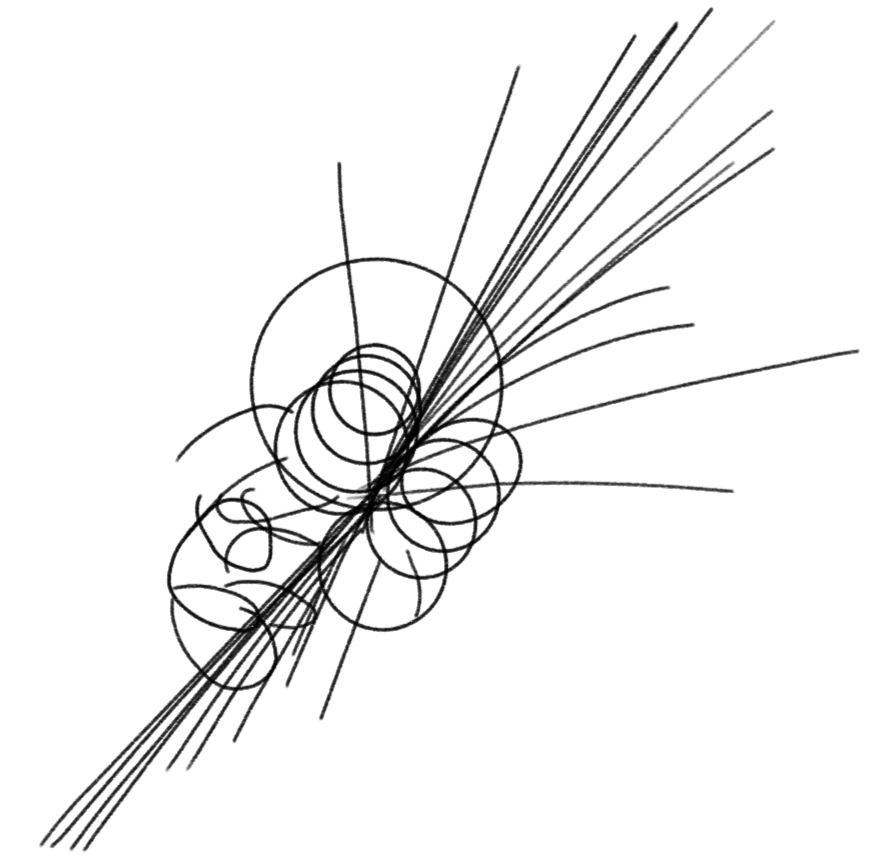
\includegraphics[width=0.5\linewidth]{img/particle_detector.png}
    \caption{Particle tracks as from a bubble chamber experiment.}
    \label{fig:particle_detector}
\end{figure}

Other efforts, such as VERITAS (Very Energetic Radiation Imaging Telescope Array System), are large telescope observatories located at the surface of the Earth. VERITAS detects the high energy gamma rays (in the 10$^9$-10$^{12}$ eV energy range) to further study astronomical objects like supernovae, pulsars, and black holes, which emit these highest energy forms of light.



\subsection{Black Holes}

Black holes are fascinating objects to study. Though marvelously simple in their construction, they are beaming with some of the most exotic physical phenomena the Universe has to offer. They defy our common understanding of many fundamentals, like space, time, mass and energy (to name a few). There are many ways to go about defining exactly what a black hole is. I will try to offer you a few different ways of conceptualizing what I am talking about.

Colloquially, it is sometimes said that black holes are where all known laws of physics go to die. Though I will concede that indeed, classical physics (think Newtonian, i.e. $\vec{F}=m\vec{a}$) becomes wholly inadequate to describe what is going on there, overall, black holes are very simple. Astrophysical black holes can be condensed down to 2 fundamental properties: how heavy they are, and how fast they spin. That's it! Now, lots of weird stuff can and does happen around them, but mass and spin is all there is to it! 
Black holes do not have what we could consider to be a ``proper'' surface, but as you get closer and closer to their center, you can reach a point where their gravitational pull is so strong that not even light can escape! This forms an apparent surface called the event horizon.

\begin{figure}[h!]
    \centering
    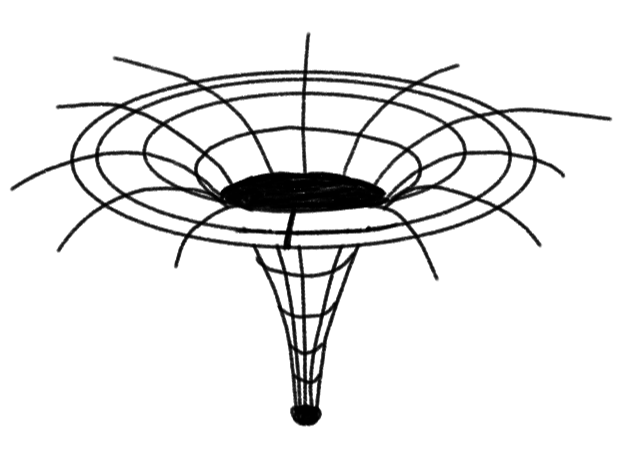
\includegraphics[width=0.6\linewidth]{img/bh.png}
    \caption{Black holes warp the very fabric of spacetime.}
    \label{fig:bh}
\end{figure}

Now, we know that one way to end up with a black hole is to have a star so massive that it ends up collapsing under its own weight. And we also know that the most massive objects in the Universe cannot be anything other than black holes (not counting composite structures, like galaxies, which are a collection of thousands to millions of stars). Supermassive black holes weigh somewhere in the neighborhood of millions to billions of times the mass of our Sun! But! A high mass is not a requirement to produce a black hole. Instead, what defines them is how prodigiously concentrated their matter content is. Nothing precludes us from finding a black hole that weighs as little as you: it would just be incredibly small! There is a common misconception of a black hole as some sort of cosmic vacuum cleaner, when in reality, black holes follow the exact same rules as every other thing in the Universe! Were we to replace the Sun with a similarly heavy black hole, nothing would meaningfully change for us -- but we would start to miss the warmth of sunlight pretty quickly.


\subsubsection{An Introduction to General Relativity}
The very idea of a black hole first arose in 1916 as a straightforward solution to Einstein's equations for gravity and spacetime. You might have heard of those equations referred to as the theory of General Relativity. Its foundational tenets are actually quite simple in essence.

Space and time are intertwined into a fabric aptly referred to as ``spacetime.'' In concrete terms, this simply means that everything that ever was or ever will be can be placed on a 4-dimensional grid, described by 4 coordinates: time $t$, and position $(x, y, z)$. 
Though this grid is flat by default, matter distorts spacetime and makes it curve inwards. Straight lines start bending towards the places where matter is most concentrated. The physical manifestation of this idea is what we call gravity. General relativity tells us that we humans exist on the surface of the Earth, not because it acts as a giant magnet on us, but because its mass is bending space and time around it -- and we just happen to be there to feel it! Now, luckily for us, the Earth isn't too heavy compared to other cosmic objects, so the surface forces under our feet are enough to keep us aground. However, the gravitational field of objects like black holes is such that there exists no other force in the entirety of the Universe that can counteract it! That's what we mean when we talk of \textit{gravitational collapse}.


\subsubsection{Supermassive Black Holes}

A fun fact is that most sufficiently massive galaxies are hosts to supermassive black holes, snugly located at their centers: gargantuan monsters whose masses can exceed millions to tens of billions times that of our Sun. They act as superengines, powering entire galaxies through prodigiously energetic processes. A certain fraction of them are actually so luminous that astronomers have taken to calling them AGNs, for Active Galactic Nuclei, as they have sometimes been observed to outshine entire galaxies!

Now, you heard me right, I just called a black hole \textit{luminous}. That is not a misnomer, or a mistake, or even some vague metaphor. Though you might remember from above that, indeed, black holes themselves might not allow light to escape from their surface and therefore appear completely dark, all you need to ``see'' them is to place them in gas-rich environments, where you can trigger a process called accretion. Through accretion, surrounding matter gets gravitationally locked onto tight orbits around the black hole, and is slowly stripped of its energy as it falls onto the black hole -- releasing it in the form of light! Now, matter does not plunge directly into the black hole, because of conservation of angular momentum. What happens is that gas particles usually come in with some initial tangential velocity (perpendicular to the line between the point object and black hole), which is conserved even as their radial velocity (directly towards the black hole) precipitates them towards annihilation. Those particles will form spiral trajectories through what we call an \textit{accretion disk}. Now, through friction and a number of other more complicated processes, energy is released as radiation. It begins with thermal radiation, which, for accretion disks, will usually peak in the UV, or ultraviolet. Any matter with any temperature at all emits thermal radiation, even you! Though, people are quite a bit colder than the matter surrounding a black hole, so the light we emit is much less energetic, and instead peaks in the IR, or infrared, which we cannot see with our naked eyes. Some of those UV photons are going to collide with very, \textit{very} hot electrons (with a temperature around $10^9$ $^\circ \mathrm{F}$) and get kicked into the even more energetic domain (this time, into the X-ray!). This X-ray light signal is very particular and is what we can observe with our space-based telescopes, like Chandra or (in the near future, hopefully) XRISM, STROBE-X, Athena, HEX-P, etc.






\subsection{Numerical Relativity \& Gravitational Waves}

Historically, our understanding of the universe has heavily relied on what we can learn from light (formally known as electromagnetic radiation). We can see some of this light when we look up to the skies on a dark night, but we can also observe the universe in types of light that human eyes can't detect. X-rays, microwaves, and radio waves are all forms of electromagnetic radiation just like visible light, and we can use these types of radiation to learn about the universe. In addition to light, another way we have learned about the universe is by detecting astrophysical particles like we've described in the sections above. 

In 2015, we opened an entirely new window to the universe by detecting a completely separate form of radiation -- gravitational radiation, more commonly called gravitational waves. This form of radiation was predicted by Albert Einstein in 1916, and it was finally detected 99 years later by an experiment called LIGO, the Laser Interferometer Gravitational-Wave Observatory.

So, what are gravitational waves? They are ripples in the fabric of space and time, just like the waves you see in a pond when you toss a pebble. But instead of traveling through water, the waves travel through space itself and are created by some of the most powerful events in the universe. Let's think about this analogy in a bit more detail. The surface of a pond reacts differently when we move different objects across it - bigger objects create bigger ripples. The same thing is true in space! Heavier objects will cause space to distort and bend more, meaning the gravitational waves they produce will be larger.


\subsubsection{Gravitational Wave Sources}

Every object moving in space can produce gravitational waves. However, you need a super massive object or energetic event to distort the fabric of space time enough to create a detectable gravitational wave signal. So when we detect astrophysical gravitational waves on Earth, they must be coming from cataclysmic events. The first signal we detected in 2015 came from two black holes that had been orbiting around each other for millions of years. In the final seconds before they collided and merged with each other, the two black holes were moving so quickly that they produced huge gravitational wave ripples that stretched and squeezed space itself. These ripples propagated across the universe, passing through Earth and stretching and squeezing our planet and the LIGO detectors on it. These distortions happened to us as well, so on that day everyone and everything on our planet was stretched and squeezed! However, since the colliding black holes were so far away, the gravitational wave ripples that passed through Earth were so small that the planet was only distorted by 1/1000th the size of a proton! 

It is important to note that we can study these sources by measuring them with detectors, or we can consider them in a theoretical and computational context. Numerical relativity is particularly useful for studying the merger of two astrophysical objects (such as black holes or, in more exotic scenarios, boson stars). This involves running a simulation on a powerful computer which, as the name implies, simulates the two objects on their trajectories. This is done by solving the field equations - the equations which describe the system - iteratively. One way to set up this simulation is called a 3+1 formalism, which separates the 3 spatial dimensions and iterates over the 1 time dimension. The output of a numerical relativity simulation can then be used to model real systems or to inform our understanding of as-of-yet undetected objects.

Merging black holes are not the only sources that emit detectable gravitational waves. Binary neutron star (BNS) mergers, and potentially nearby supernovae, can also produce gravitational waves within the frequency range detectable by instruments like LIGO. In addition, other astrophysical sources can create gravitational wave signals in frequencies that LIGO cannot detect. For these sources, we can turn to the Laser Interferometer Space Antenna (LISA), as discussed in the next section. LISA is designed to observe supermassive black hole binaries in different frequency bands, providing a new window to the universe's gravitational wave landscape. This range of frequencies for different GW sources is called the gravitational wave spectrum, and it is a parallel to the electromagnetic spectrum that we introduced earlier.


\begin{figure}
    \centering
    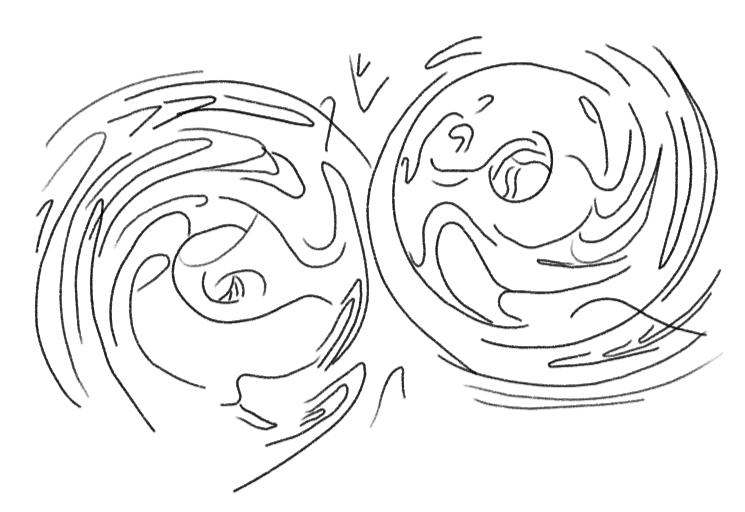
\includegraphics[width=0.8\linewidth]{img/stylized_bbh.png}
    \caption{A binary pair of black holes -- such configurations may give rise to gravitational waves that are detectable by instruments like LIGO.}
    \label{fig:stylized_bbh}
\end{figure}

\subsubsection{GW Detectors}

For a long time, scientists were unsure whether or not gravitational waves were a truly physical phenomena. Some believed they were the result of a choice of coordinates, and others were troubled by the implication of a singularity in the relevant equations. Feynman famously argued gravitational waves were indeed physical because they would do ``work'' and thus would be expected to transmit energy. This not only convinced his colleagues it would make sense to think of gravitational waves physically, but suggested a means of detecting them.

Current gravitational wave detectors (observatories such as LIGO-Kagra-Virgo) measure the distortion of space-time that results from a gravitational wave passing through. The distortions correspond to two types of polarization, called ``plus'' and ``cross'' which describe how the wave moves the spacetime as it passes through. If you imagine a flat circle of many points, you can think of the plus polarization as making these points oscillated up/down and left/right, where cross would produce oscillates along the diagonals. From these distortions, we are able to calculate how much energy is transferred by the gravitational wave, and infer information about the systems which produced it.

Detections are made within a range of frequencies over which the detector is sensitive, that is, the frequencies fall within ``sensitivity curves'' which differ between detectors. The primary constraint in measuring a gravitational wave using a particular detector is whether the signal measured can be isolated from the noise the data contains. This ratio of signal to noise is what determines the detector sensitivity band. You may wonder whether you can hear such a signal, and indeed you can (disclaimer: once it has been scaled to human hearing ranges). If you search online for LIGO chirp audio, you can hear the sound of a binary black hole merger!

You may know from reading about more traditional observatories that signals can be distorted by things such as the atmosphere or nearby light pollution. In the case of gravitational wave detectors, we are susceptible to many auditory distortions, such as from earthquakes or even small animals rummaging near the tunnels. In order to get better data, scientists and engineers are working on launching a space-based observatory, called LISA for ``Laser Interferometer Space Antenna''. Based on current projections, LISA should launch around 2037. By comparing signals that are measured by LIGO-Kagra-Virgo and LISA, as well as the future Einstein Telescope and Cosmic Explorer, scientists will be able to develop a better understanding of our universe.

\begin{figure}
    \centering
    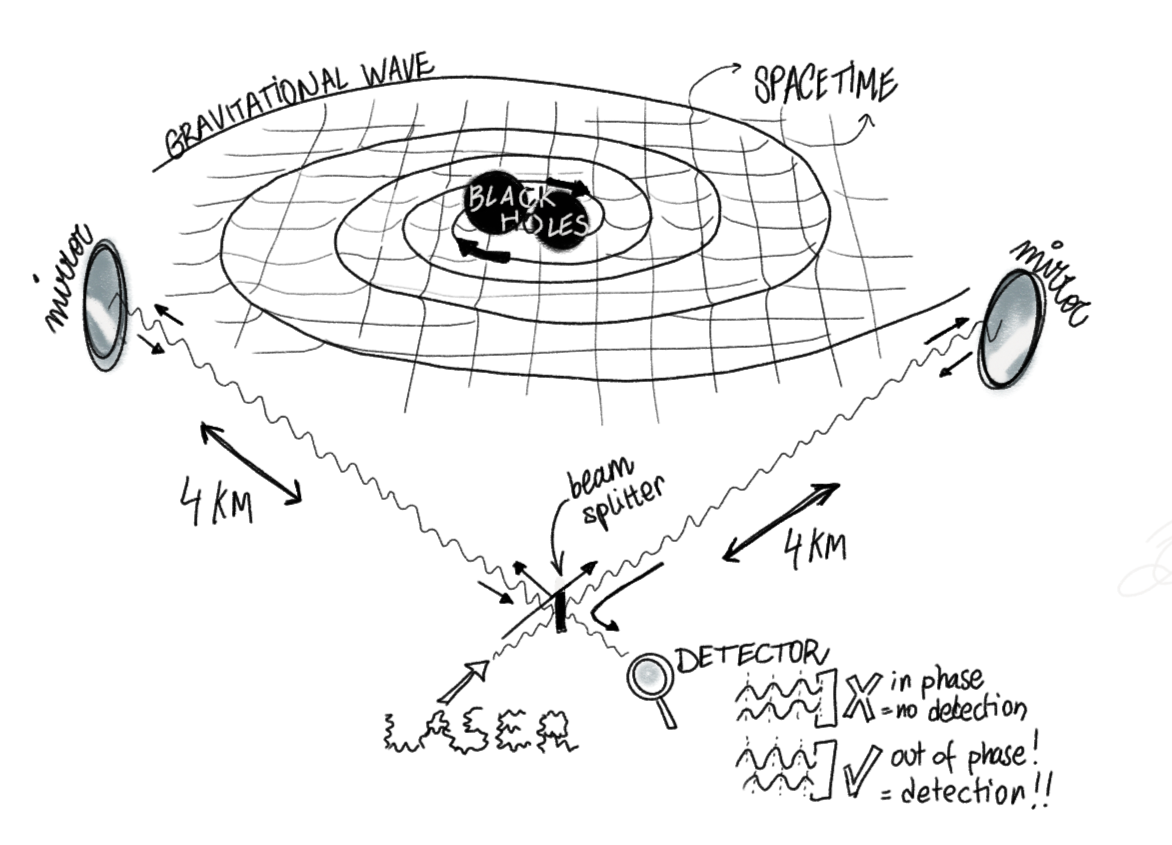
\includegraphics[width=1\linewidth]{img/ligo.png}
    \caption{Schematic of the LIGO-Kagra-Virgo gravitational wave interferometer showing detection scenario from a black hole binary system.}
    \label{fig:ligo}
\end{figure}